\section{Tholston}\label{tholston}

Tags: NPC Alias: Il Viscido Creatore: Davide Razza: Umano

\section{Tholsthon}\label{tholsthon}

\begin{center}\rule{0.5\linewidth}{0.5pt}\end{center}

\begin{figure}
\centering

\includegraphics{Mestesso94_A_fat_male_elf_with_a_an_opulent_dress_and_a_red_rin_c74dd3a8-e6aa-4e35-b14d-b115230870f5.png}
\caption{Mestesso94\_A\_fat\_male\_elf\_with\_a\_an\_opulent\_dress\_and\_a\_red\_rin\_c74dd3a8-e6aa-4e35-b14d-b115230870f5.png}
\end{figure}

Informazioni Generali

Anno di nascita: 1958

Paese di nascita: Azura

Razza: Umano

Relazioni:

Alleati:

Nemesi:

Possedimenti importanti:

\begin{center}\rule{0.5\linewidth}{0.5pt}\end{center}

\subsection{1. Descrizione Generale}\label{descrizione-generale}

\begin{center}\rule{0.5\linewidth}{0.5pt}\end{center}

\begin{figure}
\centering
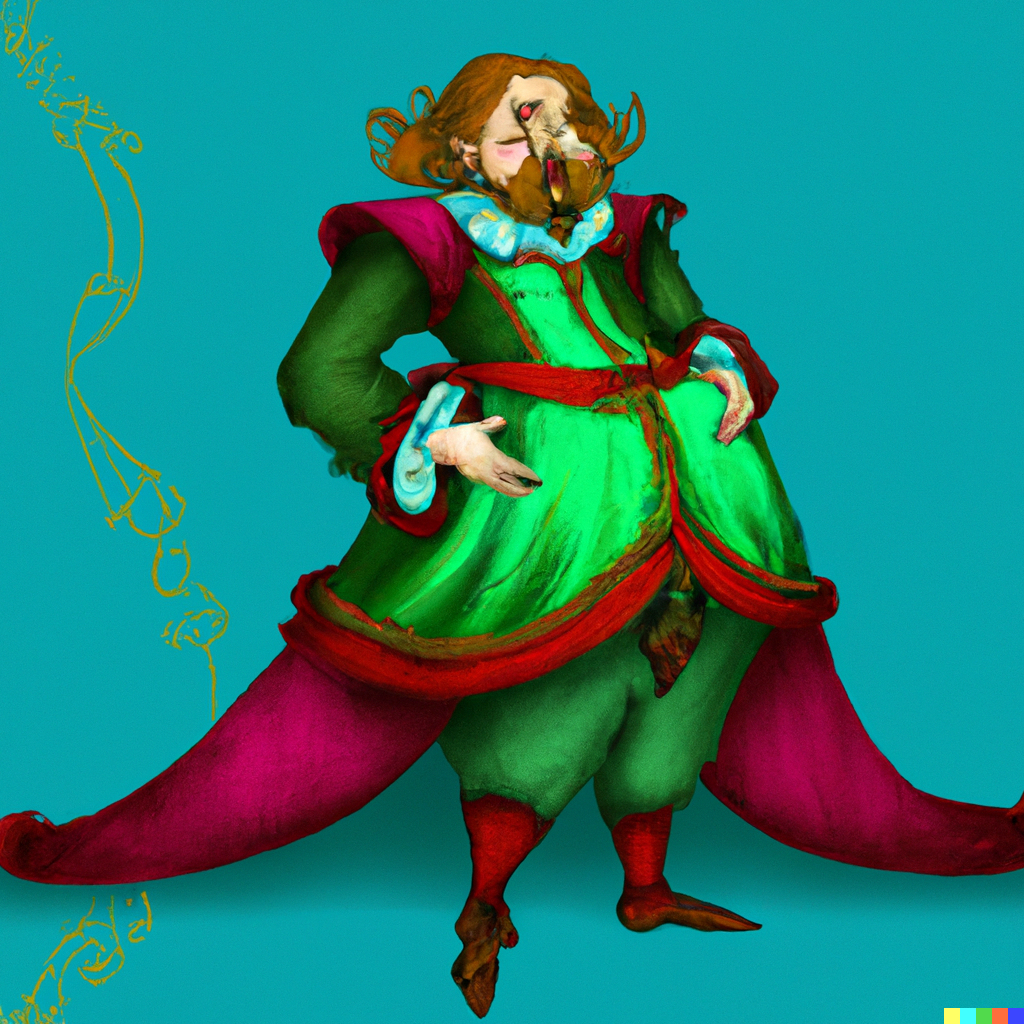
\includegraphics{DALLE_2023-03-26_16.17.47_-_A_fat_elf_with_a_an_opulent_dress._fantasy_setting_cartoon_style.png}
\caption{DALL·E 2023-03-26 16.17.47 - A fat elf with a an opulent dress.
fantasy setting, cartoon style.png}
\end{figure}

Tholsthon è un uomo obeso e viscido dall'aspetto poco attraente. Ha la
pelle grassa e sudata, e il suo viso rotondo è sempre coperto di un
sottile strato di sudore. I suoi capelli sono sempre pettinati con cura.
Tuttavia, nonostante il suo aspetto poco attraente, Tholsthon indossa
gioielli e abiti costosi e fa di tutto per ostentare la sua grande
ricchezza.

Attualmente ricopre la prestigiosa carica di Ministro dell'Economia
della città di
\href{Azura\%207c14164a934a40648d94bf415b52eee0.md}{Azura}

\subsection{2. Biografia}\label{biografia}

\begin{center}\rule{0.5\linewidth}{0.5pt}\end{center}

Tholsthon è nato in una famiglia povera e ha dovuto lottare duramente
per ottenere ciò che voleva nella vita. Fin da giovane, ha dimostrato di
avere un talento innato per gli affari e ha iniziato a fare piccoli
investimenti che gli hanno permesso di accumulare qualche soldo.

Tholsthon ha poi deciso di sfruttare le sue abilità imprenditoriali per
fare soldi in modo più consistente, e ha aperto una serie di attività
commerciali che gli hanno fruttato ingenti guadagni. Tuttavia, non è mai
stato del tutto onesto nei suoi affari, spesso facendo ricorso a trucchi
e imbrogli per guadagnare denaro.

Nonostante questo, Tholsthon ha guadagnato una certa reputazione come
imprenditore di successo, e quando la posizione di ministro
dell'economia di Azura si è resa vacante, Tholsthon ha deciso di
candidarsi per il posto. Ha usato la sua influenza e i suoi contatti per
fare pressione sui membri del consiglio della città, e alla fine è
riuscito a farsi eleggere come ministro dell'economia.

Una volta in carica, Tholsthon ha iniziato a sfruttare la sua posizione
per arricchirsi ulteriormente, stringendo accordi con commercianti
corrotti e rubando fondi pubblici. Ha anche fatto in modo che le sue
attività personali fossero sempre al primo posto, persino a discapito
della popolazione.

Tuttavia, nonostante i suoi metodi poco ortodossi, Tholsthon ha
continuato a mantenere la sua posizione di potere grazie alla sua
astuzia e alla sua capacità di manipolare le persone intorno a lui. Oggi
è considerato uno degli uomini più potenti di Azura, ma anche uno dei
più odiati e temuti.

A causa delle sue attività illecite e nascoste Tholsthon si trova spesso
coinvolto in situazioni poco raccomandabili. È infatti spesso vittima di
furti e rapimenti, ma fa di tutto per non farlo scoprire alla
popolazione per paura di perdere fama e potere.

\begin{quote}
``Ti pago se mi lasci andare'' - Tipica proposta di Tholsthon quando si
trova in difficoltà
\end{quote}

\subsection{3. Carriera}\label{carriera}

\begin{center}\rule{0.5\linewidth}{0.5pt}\end{center}

Dopo aver fatto fortuna nei suoi affari personali, Tholsthon ha deciso
di entrare in politica. Ha iniziato a partecipare alle riunioni del
consiglio comunale della città di Azura, dove ha fatto amicizia con
alcuni dei consiglieri più influenti. Grazie alle sue capacità
persuasive e alla sua astuzia, è riuscito a farsi eleggere come
consigliere della città.

Da consigliere, Tholsthon ha lavorato duramente per farsi notare dai
suoi colleghi, presentando proposte di legge innovative e dimostrando di
avere una buona comprensione delle questioni economiche. Grazie alla sua
esperienza nel mondo degli affari, Tholsthon ha iniziato a farsi un nome
come esperto di economia e finanza, e la sua reputazione è cresciuta
rapidamente.

Dopo qualche anno come consigliere, Tholsthon ha deciso di candidarsi
per il ruolo di assessore alle finanze della città di Azura. Grazie alle
sue abilità imprenditoriali e alla sua conoscenza del sistema
finanziario, è riuscito a farsi eleggere con una maggioranza
schiacciante.

Come assessore alle finanze, Tholsthon ha dimostrato di avere una grande
abilità nel gestire i soldi pubblici e ha fatto risparmiare alla città
ingenti somme di denaro. Questo gli ha permesso di guadagnarsi la stima
e la fiducia dei suoi colleghi, che lo hanno visto come un leader in
grado di fare la differenza.

Grazie a queste esperienze politiche, Tholsthon è riuscito infine a
farsi eleggere come ministro dell'economia della città di Azura, una
posizione che gli ha dato un potere enorme sulle decisioni economiche
della città e sulle scelte riguardanti il commercio. Tuttavia, come
abbiamo visto in precedenza, Tholsthon ha spesso usato questa posizione
per il suo beneficio personale, arricchendosi a discapito della
popolazione.

\subsection{4. Personalità}\label{personalituxe0}

\begin{center}\rule{0.5\linewidth}{0.5pt}\end{center}

Tholsthon è un uomo avido e egoista, che vede solo il proprio profitto e
il proprio potere. È noto per la sua mancanza di scrupoli, e non esita a
usare metodi illegali o immorali per raggiungere i suoi obiettivi.
Tholsthon è anche molto vanitoso e si vanta della sua grande ricchezza,
ostentando gioielli costosi e abiti lussuosi.

\begin{center}\rule{0.5\linewidth}{0.5pt}\end{center}

\subsection{A. Coinvolgimenti in eventi
recenti}\label{a.-coinvolgimenti-in-eventi-recenti}

\begin{center}\rule{0.5\linewidth}{0.5pt}\end{center}

\href{Untitled\%20Database\%209f53e1bff1174ede884f4b52cee86e8c.csv}{Untitled
Database}

\subsection{B. Aggiornamenti}\label{b.-aggiornamenti}

\begin{center}\rule{0.5\linewidth}{0.5pt}\end{center}

\href{Untitled\%20d9e5fb5b7a0042f9b99de48e09e1a7c6.csv}{}
